\documentclass{article}
\usepackage{booktabs}
\usepackage{amsmath}
\usepackage{amssymb}
\usepackage[noend]{algorithmic}
\usepackage[nothing]{algorithm}
\usepackage{tikz}
\usepackage{latexsym}
\usepackage{float}
\providecommand{\e}[1]{\ensuremath{\times 10^{#1}}}
\renewcommand{\thealgorithm}{}
\title{CS 522: Data Structures and Algorithms II \\ Homework 1}
\author{Dustin Ingram}
\begin{document}
\maketitle
\begin{enumerate}
    \item \textbf{Solution:}
    If both \textsc{Increment} and \textsc{Decrement} operations were included
    in the $k$-bit counter, an amortized analysis of the cost of $n$ operations
    would cost as much as $\Theta(nk)$ time because we would no longer be able
    to consider each operation as a consecutive \textsc{Increment}, but rather
    as any combination of \textsc{Increment}s and \textsc{Decrement}s. Thus, in
    a worse-case scenario, it would be possible to alternate $n$ times between
    two operations which cost $O(k)$ each, resulting in a total cost of
    $\Theta(nk)$.

    \item \textbf{Solution:}
    To show that the amortized cost of \textsc{Table-Delete} under this strategy
    is bounded above by a constant, we will consider two cases. We will use the
    potential function:

    $$ \Phi(T) = | 2\cdot T.num - T.size | $$

    The first case is the one in which the table does not contract, and thus
    $num_{i} = num_{i-1}-1$, $size_{i} = size_{i-1}$, and $c_{i} = 1$:

    \begin{align*}
        \hat{c_{i}} &= c_{i} + \Phi_{i} - \Phi_{i-1} \\
        \hat{c_{i}} &= 1 + |2\cdot num_{i} - size_{i}| - | 2\cdot num_{i-1} - size_{i-1} | \\
        \hat{c_{i}} &= 1 + |2\cdot(num_{i-1} - 1) - size_{i-1}| - | 2\cdot num_{i-1} - size_{i-1} | \\
        \hat{c_{i}} &= 1 + |-2| \\
        \hat{c_{i}} &= 3 \\
    \end{align*}

    The second case is the one in which the table does contract, and thus
    $size_{i} = \frac{2}{3}size_{i-1}$, $num_{i-1} = \frac{1}{3}size_{i-1}$, and
    $c_{i} = num_{i} + 1$:

    \begin{align*}
        \hat{c_{i}} &= c_{i} + \Phi_{i} - \Phi_{i-1} \\
        \hat{c_{i}} &= (num_{i} +1) + |2\cdot num_{i} - size_{i}| - | 2\cdot num_{i-1} - size_{i-1} | \\
        \hat{c_{i}} &= ((num_{i-1} - 1) + 1) + |2\cdot(num_{i-1} - 1) - \frac{2}{3}size_{i-1}| - | 2\cdot num_{i-1} - size_{i-1} | \\
        \hat{c_{i}} &= (num_{i-1}) + |-2 + \frac{1}{3}size_{i-1}| \\
        \hat{c_{i}} &= 2 \\
    \end{align*}

    Thus we see that the amortized cost of \textsc{Table-Delete} is at most 3
    and is thus bounded.

    \item \textbf{Solution:}
    As follows:
    \begin{figure}[H]
    \centering
    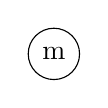
\begin{tikzpicture}[
      level 1/.style={sibling distance=48mm, level distance=10mm},
      level 2/.style={sibling distance=16mm, level distance=10mm},
      level 3/.style={sibling distance=8mm, level distance=10mm},
    ]
    \node [circle,draw, minimum height=.5cm, minimum width=.5cm] (1){m};
    \end{tikzpicture}
    \end{figure}

    \begin{figure}[H]
    \centering
    \begin{tikzpicture}[
      level 1/.style={sibling distance=48mm, level distance=10mm},
      level 2/.style={sibling distance=16mm, level distance=10mm},
      level 3/.style={sibling distance=8mm, level distance=10mm},
    ]
    \node [circle,draw, minimum height=.5cm, minimum width=.5cm] (1){m};
    \node [circle,draw, minimum height=.5cm, minimum width=.5cm, right of=1] (2){m-1};
    \path [line] (1)--(2);
    \end{tikzpicture}
    \end{figure}

    \begin{figure}[H]
    \centering
    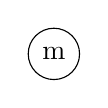
\begin{tikzpicture}[
      level 1/.style={sibling distance=48mm, level distance=10mm},
      level 2/.style={sibling distance=16mm, level distance=10mm},
      level 3/.style={sibling distance=8mm, level distance=10mm},
    ]
    \node [circle,draw, minimum height=.5cm, minimum width=.5cm] (1){m};
    \end{tikzpicture}
    \end{figure}

    \begin{figure}[H]
    \centering
    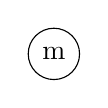
\begin{tikzpicture}[
      level 1/.style={sibling distance=48mm, level distance=10mm},
      level 2/.style={sibling distance=16mm, level distance=10mm},
      level 3/.style={sibling distance=8mm, level distance=10mm},
    ]
    \node [circle,draw, minimum height=.5cm, minimum width=.5cm] (1){m};
    \end{tikzpicture}
    \end{figure}

    \begin{figure}[H]
    \centering
    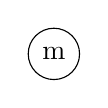
\begin{tikzpicture}[
      level 1/.style={sibling distance=48mm, level distance=10mm},
      level 2/.style={sibling distance=16mm, level distance=10mm},
      level 3/.style={sibling distance=8mm, level distance=10mm},
    ]
    \node [circle,draw, minimum height=.5cm, minimum width=.5cm] (1){m};
    \end{tikzpicture}
    \end{figure}

    \begin{figure}[H]
    \centering
    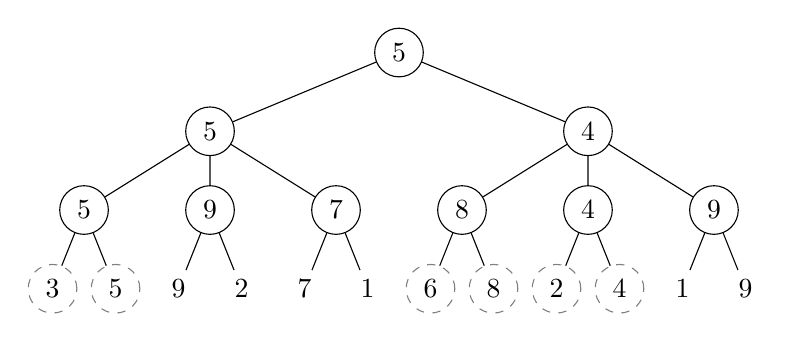
\begin{tikzpicture}[
      level 1/.style={sibling distance=48mm, level distance=10mm},
      level 2/.style={sibling distance=16mm, level distance=10mm},
      level 3/.style={sibling distance=8mm, level distance=10mm},
    ]
    \node [circle,draw, minimum height=.5cm, minimum width=.5cm] (z){5}
      child {node [circle,draw] (a) {5}
        child {node [circle,draw] (b) {5}
          child {node [circle, dashed, draw=gray] (3) {3}}
          child {node [circle, dashed, draw=gray] (5) {5}}
        }
        child {node [circle,draw] (c) {9}
          child {node (9) {9}}
          child {node (2) {2}}
        }
        child {node [circle,draw] (d) {7}
          child {node (7) {7}}
          child {node (1) {1}}
        }
      }
      child {node [circle,draw] (j) {4}
        child {node [circle,draw] (k) {8}
          child {node [circle, dashed, draw=gray] (6) {6}}
          child {node [circle, dashed, draw=gray] (8) {8}}
        }
        child {node [circle,draw] (l) {4}
          child {node [circle, dashed, draw=gray] (2) {2}}
          child {node [circle, dashed, draw=gray] (4) {4}}
        }
        child {node [circle,draw] (m) {9}
          child {node (1) {1}}
          child {node (9) {9}}
        }
    };
    \end{tikzpicture}
    \end{figure}


    \item \textbf{Solution:}

    \item \textbf{Solution:}

    \item \textbf{Solution:}

    \item \textbf{Solution:}

    \item \textbf{Solution:}
\end{enumerate}
\end{document}
